% !TeX spellcheck = de_DE
\chapter{Elektronikdesign und Hardware-Architektur}
\label{sec:elektrisches_H}

Dieses Kapitel beschreibt die Konzeptionierung, Komponentenauswahl und das Platinendesign (PCB) für die Steuerung des 6-DOF-Roboterarms. Die zu entwickelnde Platine fungiert als zentrales Management-System des Roboters. Sie nimmt die High-Level-Befehle des Raspberry Pi 4B entgegen, verarbeitet diese auf einem STM32F446RET6-Chip und steuert über eine dedizierte Leistungselektronik sechs TMC5160T Pro v1.0 Schrittmotortreiber an. Neben der Signalintegrität steht die stabile Spannungsversorgung der NEMA-17-Motoren im Vordergrund.

\section{Systemarchitektur und Signalfluss}
\label{subsec:systemarchitektur}
In diesem Abschnitt wird das grundlegende Blockschaltbild der Elektronik beschrieben. Das System teilt sich in drei logische Ebenen auf: High-Level-Recheneinheit (Raspberry Pi), Low-Level-Steuerung (STM32) und die Leistungsebene (TMC5160T Treiber). Die Kommunikation erfolgt über UART (Pi zu STM32) und einen gemeinsamen SPI-Bus für die Konfiguration der Treiberstufen.

\begin{figure}[htbp]
	\centering
	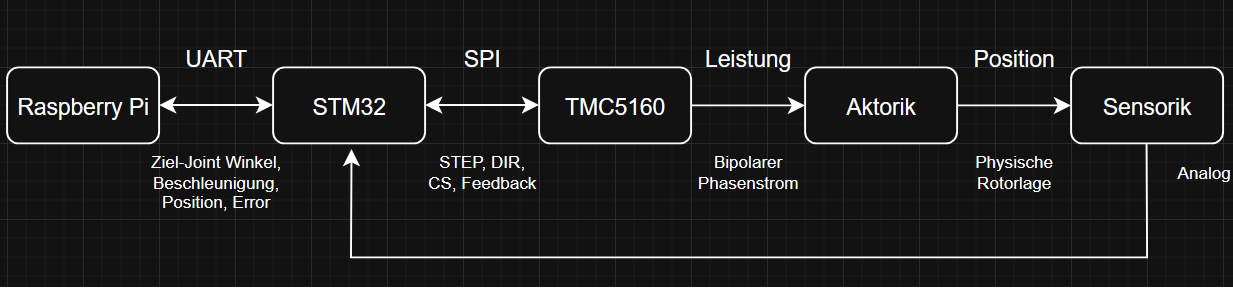
\includegraphics[width=0.9\textwidth]{figures/allgemein/blockschaltbild.png}
	\caption{Blockschaltbild der Elektronik-Architektur}
\end{figure}
\cite{a2021_this}

\section{Komponentenauswahl und Begründung}
\label{subsec:komponentenauswahl}

\subsection{Zentraler Mikrocontroller (STM32F446RET6)}
Die Wahl fiel auf den STM32F446RET6 im LQFP64-Gehäuse. Ausschlaggebend hierfür waren die hohe Taktfrequenz von 180\,MHz sowie das Vorhandensein von ausreichend Hardware-Timern, um sechs Schrittmotoren unabhängig und synchron per Hardware-PWM anzusteuern (siehe \ref{subsec:hal_STEP}). Zudem bietet der Chip genügend GPIOs für die sechs separaten Chip-Select-Leitungen des SPI-Busses.

\subsection{Schrittmotortreiber (TMC5160T Pro v1.0)}
Für die Ansteuerung der NEMA-17-Schrittmotoren werden TMC5160T Pro v1.0 Module genutzt. Diese Treiber bieten neben einer hohen Stromtragfähigkeit vor allem die Anbindung über einen geteilten SPI-Bus, was eine dynamische Konfiguration der Motorströme erlaubt.

\section{Mikrocontroller-Infrastruktur und Peripherie}
\label{subsec:mcu_infrastructure}
Für den stabilen Betrieb des STM32F446RET6 wurde eine dedizierte Infrastrukturbeschaltung auf dem Board implementiert. Diese sichert die Signalqualität, die Programmierbarkeit und optionale Diagnosemöglichkeiten.

\subsection{Taktversorgung (HSE) und Reset-Schaltung}
Um die harten Echtzeitanforderungen bei der synchronen Generierung der Schrittfrequenzen zu erfüllen, wird der interne RC-Oszillator des STM32 durch einen präzisen, externen Quarzoszillator (High-Speed External, HSE) ersetzt. Dieser ist mit zwei Lastkondensatoren (\texttt{C10}, \texttt{C11}) und einem Serienwiderstand (\texttt{R3}) beschaltet. Die manuelle Systemrücksetzung wird über einen physischen Taster realisiert, der über ein RC-Glied hardwareseitig entprellt ist, um transiente Störungen auf der \texttt{NRST}-Leitung zu blockieren.

\subsection{Programmierschnittstelle (SWD) und USB-C-Interface}
Das Flashen und Debuggen der Firmware erfolgt über ein standardisiertes Serial-Wire-Debug-Interface (SWD) via Stecker \texttt{J2} (\texttt{SWDIO}, \texttt{SWCLK}). Ergänzend wurde ein USB-C-Anschluss (\texttt{J1}) als USB-2.0-Full-Speed-Schnittstelle integriert. Um eine korrekte Erkennung an modernen USB-C-Host-Anschlüssen (z.\,B. PCs) zu gewährleisten, sind die Configuration-Channel-Leitungen (\texttt{CC1}, \texttt{CC2}) mit zwei Pull-Down-Widerständen gegen Masse gezogen. Ein Pull-Up-Widerstand an der \texttt{D+}-Leitung sorgt für die korrekte USB-Enumeration.
\cite{power}

\section{Schnittstellen und Bus-Topologie}
\label{subsec:schnittstellen}

\subsection{UART-Interface zum Raspberry Pi}
Die Kommunikation mit dem Raspberry Pi erfolgt über eine direkt angebundene UART-Schnittstelle. Hier werden die berechneten Ziel-Joint-Winkel in Radiant sowie die maximale Beschleunigung vom High-Level-System an den STM32 übertragen.

\subsection{SPI-Bus und Chip-Select-Logik}
Da sich alle sechs TMC5160-Treiber denselben SPI-Bus teilen (MOSI, MISO, SCK), muss jede Achse über eine eigene Chip-Select-Leitung (\texttt{CS}) exklusiv angesprochen werden.

\subsection{STEP/DIR-Leitungen und Signalintegrität}
Neben SPI benötigt jeder Treiber eine dedizierte \texttt{STEP}- und \texttt{DIR}-Leitung zur Vorgabe von Geschwindigkeit und Drehrichtung. Da diese Signale im harten Schaltbetrieb (MHz-Bereich) arbeiten, werden im Layout optionale Vorwiderstände zur Dämpfung von Signalüberschwingen eingeplant.

\section{Spannungsversorgung und Power-Management}
\label{subsec:power}

Aufgrund der hohen Eingangsspannung von $24\,\text{V}$ und den unterschiedlichen Lastanforderungen der Systemkomponenten ist der Einsatz hocheffizienter DC/DC-Abwärtswandler (Buck Converter) zwingend erforderlich. Ein linearer Spannungsregler würde bei dieser Spannungsdifferenz eine unzulässige Verlustleistung $P_{\text{loss}} = (V_{\text{in}} - V_{\text{out}}) \cdot I$ in Form von Wärme erzeugen. Das System nutzt eine kaskadierte und parallele Schaltregler-Topologie, um vier getrennte Spannungsebenen bereitzustellen:\cite{kirasich_new}

\begin{itemize}
	\item \textbf{24\,V Hauptversorgung:} Direkte Speisung der TMC5160-Leistungsstufen über den Terminal-Block \texttt{J2}.
	\item \textbf{12\,V Lüfter-Versorgung:} Erzeugt aus den $24\,\text{V}$ über einen synchronen Abwärtswandler (\texttt{U4}). Diese Schiene dient exklusiv der Versorgung von aktiven Systemlüftern, um die Abwärme der Motortreiber effektiv abzuführen.
	\item \textbf{5\,V Logik- und Pi-Versorgung:} Über den Schaltregler (\texttt{U2}) realisiert. Diese Schiene versorgt den Raspberry Pi 4B sowie die Peripheriesensorik. Die Stabilisierung erfolgt über einen LC-Ausgangsfilter.
	\item \textbf{3,3\,V Mikrocontroller-Versorgung:} Abgestuft aus der stabilen $5\,\text{V}$-Schiene mittels eines kompakten Synchron-Abwärtswandlers. Dieser versorgt den STM32-Kern sowie die Digitalstufen der TMC5160-Treiber. Zur Entkopplung hochfrequenter Störungen der Digitalschaltungen ist die analoge Versorgungsschiene (\texttt{VDDA}) über eine Ferritperle (\textit{Ferrite Bead}, \texttt{FB1}) und ein zusätzliches Filter-Netzwerk (\texttt{C6}, \texttt{C7}, \texttt{C8}) realisiert.
\end{itemize}
\cite{kirasich_new}
\section{Prototyping und Hardware-Verifikation}
\label{subsec:prototyping}
Um die theoretische Konzeptionierung sowie die Low-Level-Softwarearchitektur vor dem finalen, integrierten Platinendesign zu validieren, wurde eine modulare Evaluierungsplatine entwickelt. Als Steuerungseinheit dient in dieser Phase ein externes \textit{STM32-Nucleo}-Entwicklungsboard.

\subsection{Architektur der Testplatine}
Die Testplatine wurde als Single-Layer-Board realisiert. Sie dient als Bus- und Verteilerplatine für die sechs TMC5160T-Modulsteckplätze (\texttt{DRV\_1} bis \texttt{DRV\_6}). Die Signale für \texttt{STEP}, \texttt{DIR} und \texttt{CS} werden über Stiftleisten flexibel an das Nucleo-Board übergeben. Der SPI-Bus ist als gemeinsame Leiterbahnstruktur über alle Treiber hinweg geroutet.

\subsection{Maßnahmen zur Signalintegrität und EMV}
Da Schrittmotortreiber steile Stromflanken erzeugen, wurden auf dem Testboard gezielte EMV-Schutzmaßnahmen umgesetzt:
\begin{itemize}
	\item \textbf{Lokale Dekopplung:} Jeder Treiber verfügt über eine direkte Pufferung aus einem $100\,\mu\text{F}$ Elektrolytkondensator (transiente Spitzenströme) und einem $100\,\text{nF}$ Keramikkondensator (hochfrequente Störungen) unmittelbar am Pin \texttt{VM}.
	\item \textbf{Überspannungsschutz:} Am 24\,V-Eingang (\texttt{J2}) ist eine Suppressordiode (TVS-Diode, \texttt{D1}) platziert, welche die Gegen-EMK der Motoren beim abrupten Bremsen absorbiert.
	\item \textbf{Massive Stromschienen:} Die Versorgungsleitung für die Motorspannung wurde auf der Oberseite als großflächige, niederohmige Kupcherschiene ausgeführt, um Spannungsabfälle zu minimieren.
\end{itemize}

\section{Schaltplan und PCB-Layout (Integriertes Design)}
\label{subsec:pcb_layout}

%TODO Leiterbahnen dimesionierung und Stromtragfähigkeit zitieren: https://www.tortai-tech.com/wp-content/uploads/2023/09/IPC-2221-Generic-Standard-on-Printed-Board-Design.pdf

\subsection{Leiterbahndimensionierung und Stromtragfähigkeit}
\label{subsubsec:trace_calculation}
Für das finale Platinendesign (gefertigt über JLCPCB) müssen die Leiterbahnbreiten der Hauptstromversorgung mathematisch begründet werden, um Überhitzungen zu vermeiden. Die Berechnung der minimalen Leiterbahnbreite erfolgt nach der gängigen Industrienorm \textbf{IPC-2221}.
\cite{a1998_ipc2221}
Die grundlegende Formel für den maximal zulässigen Strom $I$ in Abhängigkeit von der Querschnittsfläche $A$ und der zulässigen Temperaturerhöhung $\Delta T$ lautet:
\begin{equation}
	I = k \cdot \Delta T^{b} \cdot A^{c}
\end{equation}

Für Außenlagen (Top-/Bottom-Layer) gelten nach IPC-2221 die Konstanten $k = 0{,}048$, $b = 0{,}44$ und $c = 0{,}725$. Umgestellt nach der benötigten Querschnittsfläche $A$ (in $\text{mils}^2$) ergibt sich:
\begin{equation}
	A = \left( \frac{I}{k \cdot \Delta T^{b}} \right)^{\frac{1}{c}}	
\end{equation}

Da die Hauptversorgungsbahn im Layout als durchgehendes Polygon mit einer Breite von ca. $10\,\text{mm}$ ausgeführt wurde, liegt das Design deutlich im sicheren Bereich.\cite{a1998_ipc2221}

\subsection{Thermisches Management}
Um einen sicheren Betrieb trotz der hohen thermischen Beanspruchung der Treiber zu gewährleisten, werden Lüfter über die Onboard-12V-Versorgung betrieben und im Gehäuse integriert. Zudem kommen Heatsinks und Thermal Vias zum Einsatz.